\documentclass[11pt,a4paper]{article}

\usepackage[T1]{fontenc}
\usepackage{lmodern}
\usepackage[english]{babel}
\usepackage{microtype}
\usepackage{amsmath,amssymb,amsthm,mathtools}
\usepackage{geometry}
\usepackage{enumitem}
\usepackage{tikz}
\usetikzlibrary{arrows.meta,positioning}
\usepackage[hidelinks]{hyperref}
\usepackage{xurl}

\geometry{a4paper,margin=24mm,headheight=14pt}
\setlength{\parindent}{0pt}
\setlength{\parskip}{4pt plus 1pt minus 1pt}
\setlist[enumerate]{leftmargin=*,topsep=2pt,itemsep=3pt}
\allowdisplaybreaks[1]

\newtheorem*{cancellation}{Theorem 3.1 (Cancellation estimate)}
\newtheorem*{bridge}{Theorem 5.1 (Product estimate across a fast bridge)}
\newtheorem*{fixedgrowth}{Proposition (maximal growth at a fixed time)}
\newtheorem*{observationdef}{Definition (Observation)}
\newcommand{\R}{\mathbb{R}}
\newcommand{\T}{\mathbb{T}}
\newcommand{\Z}{\mathbb{Z}}
\newcommand{\PP}{\mathbb{P}}
\newcommand{\EE}{\mathbb{E}}
\newcommand{\norm}[1]{\left\lVert #1\right\rVert}
\newcommand{\one}{\mathbf{1}}

\title{\vspace{-1.4em}\textbf{Positive Metric Entropy for the Standard Map}\\[4pt]
\large Definitions, the two dynamical estimates, and fixed-time growth}
\author{Reading Group UB-UPC}
\date{20 November 2026}

\begin{document}
\maketitle
\vspace{-1.2em}

\begin{abstract}
\noindent
We summarize the main definitions in Sections 1--2 of \emph{Positive Metric Entropy for the Standard Map at Large Parameters}, state and interpret Theorems 3.1 and 5.1, and give a complete elementary proof that the mean growth shortfall $e_n(K)$ tends to zero as $K\to\infty$ for each fixed $n$, before turning to the two dynamical theorems. We define observations in detail and explain the contradiction setup from Sections 6--8.
\end{abstract}

\section{The standard map and its derivative cocycle}

The standard sine map is the area-preserving diffeomorphism of $\T^2$ given by
\begin{equation}\label{eq:map}
 f_k(x,y)=\bigl(x+y+k\sin(2\pi x),\;y+k\sin(2\pi x)\bigr)\pmod{\Z^2}.
\end{equation}
Its main result asserts that for all sufficiently large $k>0$ the Kolmogorov--Sinai entropy of $f_k$ with respect to normalized Lebesgue area is positive.

Put
\begin{equation}\label{eq:params}
 K=2\pi k,\qquad M=K+4,\qquad
 \phi(q)=2q+k\sin(2\pi q),\qquad
 v(q)=\phi'(q)=2+K\cos(2\pi q).
\end{equation}
After the fixed linear change of coordinates $(x,y)\mapsto(q_i,q_{i-1})=(x,x-y)$, the map becomes
\begin{equation}\label{eq:orbit}
 q_{i+1}=\phi(q_i)-q_{i-1}\pmod1.
\end{equation}
The corresponding linearized recurrence is
\begin{equation}\label{eq:linearization}
 u_{i+1}=v(q_i)u_i-u_{i-1},\qquad
 \begin{pmatrix}u_{i+1}\\u_i\end{pmatrix}
 =A_i\begin{pmatrix}u_i\\u_{i-1}\end{pmatrix},\qquad
 A_i=\begin{pmatrix}v(q_i)&-1\\1&0\end{pmatrix}.
\end{equation}
Let $T_{a,b}(z)$ carry the linearized pair at time $a$ to that at time $b$ along the orbit of $z$. Thus
\[
 T_{a,c}=T_{b,c}T_{a,b},\qquad T_{b,a}=T_{a,b}^{-1}.
\]
Because $\det A_i=1$ and $\norm{A_i^{\pm1}}\le M$, the Euclidean operator norm satisfies
\begin{equation}\label{eq:norm-bounds}
 1\le\norm{T_{a,b}}=\norm{T_{b,a}}\le M^{|b-a|}.
\end{equation}
The equality of forward and backward norms is special to $2\times2$ matrices of determinant one, whose singular values are $D,D^{-1}$.

\section{Growth semimetrics and mean shortfalls}

\subsection*{The growth semimetric}
Define, for integers $a,b$,
\begin{equation}\label{eq:g}
 \boxed{\quad g(a,b;z)=\log_M\norm{T_{a,b}(z)}.\quad}
\end{equation}
The transfer identities imply
\begin{equation}\label{eq:semimetric}
 \begin{gathered}
  g(a,a)=0,\qquad g(a,b)=g(b,a),\\
  g(a,c)\le g(a,b)+g(b,c),\qquad
  0\le g(a,b)\le |b-a|.
 \end{gathered}
\end{equation}
Hence $g$ is a semimetric on the integers for each orbit. In particular, $g(a,b)$ measures finite-time linearized expansion in units of the maximal available rate $\log M$.

\subsection*{The expected shortfall}
Write $\EE$ for expectation with respect to normalized area on $\T^2$, and set
\begin{equation}\label{eq:en}
 \boxed{\quad e_n(K)=\EE\left[1-\frac{g(0,n;z)}{n}\right],\qquad 0\le e_n(K)\le1.\quad}
\end{equation}
Thus $e_n\approx0$ corresponds to almost-maximal finite-time growth, whereas $e_n\approx1$ corresponds to growth that is small relative to $n\log M$.

The dynamical process is stationary under integer time shifts. Indeed, $f_k$ preserves normalized area, and $(q_i,q_{i-1})$ is uniformly distributed on $\T^2$ at every fixed $i$. The positions $q_i$ are \emph{not} being assumed independent at different times.


\subsection*{The one-step critical region $E_{0,K}$}
A first geometric object to keep in mind is the region where the one-step coefficient
\[
 v(q)=2+K\cos(2\pi q)
\]
is small, namely near the \emph{critical lines}
\[
 q=\tfrac14,\qquad q=\tfrac34,
\]
for which $\cos(2\pi q)=0$. In the notes below we denote schematically by
\[
 E_{0,K}=\{(q_0,q_{-1})\in\T^2:\ |\cos(2\pi q_0)|\le \eta_K\},
\]
where $\eta_K>0$ is a small threshold depending on $K$. Thus $E_{0,K}$ is the
\emph{critical region to avoid}: it is a union of two narrow vertical strips in the
$(q_0,q_{-1})$-torus representation. Its complement is the region where the coefficient
$|v(q_0)|$ is large, and there one has the familiar forward-invariant cone field for the
one-step derivative.

\begin{figure}[htbp]
\centering
\begin{minipage}[c]{0.50\textwidth}
\centering
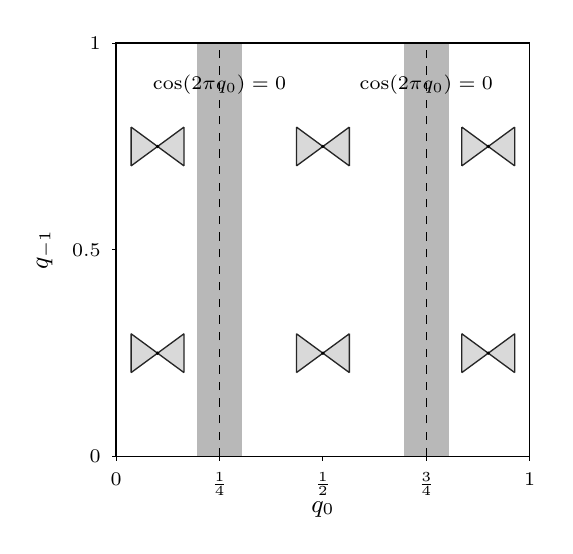
\begin{tikzpicture}[x=5.25cm,y=5.25cm]
  \def\eta{0.055}
  \fill[white] (0,0) rectangle (1,1);
  \fill[black!28] ({0.25-\eta},0) rectangle ({0.25+\eta},1);
  \fill[black!28] ({0.75-\eta},0) rectangle ({0.75+\eta},1);
  \draw[line width=0.6pt] (0,0) rectangle (1,1);
  \foreach \x/\lab in {0/0,0.25/\frac14,0.5/\frac12,0.75/\frac34,1/1}{
    \draw (\x,0) -- ++(0,-0.010);
    \node[below,font=\scriptsize] at (\x,-0.016) {$\lab$};
  }
  \foreach \y in {0,0.5,1}{
    \draw (0,\y) -- ++(-0.010,0);
    \node[left,font=\scriptsize] at (-0.014,\y) {$\y$};
  }
  \draw[dashed] (0.25,0) -- (0.25,1);
  \draw[dashed] (0.75,0) -- (0.75,1);
  \node[below,font=\small] at (0.5,-0.085) {$q_0$};
  \node[above,rotate=90,font=\small] at (-0.13,0.5) {$q_{-1}$};
  \node[font=\scriptsize,align=center] at (0.25,0.90) {$\cos(2\pi q_0)=0$};
  \node[font=\scriptsize,align=center] at (0.75,0.90) {$\cos(2\pi q_0)=0$};
  % Each invariant cone is drawn as a double cone (an hourglass):
  % two opposite sectors of the tangent plane sharing one vertex.
  \foreach \x in {0.10,0.50,0.90}{
    \foreach \y in {0.25,0.75}{
      \begin{scope}[shift={(\x,\y)}]
        \fill[black!15] (-0.064,-0.047) -- (0,0) -- (-0.064,0.047) -- cycle;
        \fill[black!15] ( 0.064,-0.047) -- (0,0) -- ( 0.064,0.047) -- cycle;
        \draw[black!85,line width=0.48pt]
          (-0.064,-0.047) -- (0,0) -- (-0.064,0.047)
          (-0.064,-0.047) -- (-0.064,0.047);
        \draw[black!85,line width=0.48pt]
          ( 0.064,-0.047) -- (0,0) -- ( 0.064,0.047)
          ( 0.064,-0.047) -- ( 0.064,0.047);
        \fill[black] (0,0) circle[radius=0.0043];
      \end{scope}
    }
  }
\end{tikzpicture}
\end{minipage}%
\hfill
\begin{minipage}[c]{0.45\textwidth}
\raggedright
\textbf{Schematic picture of $E_{0,K}$.}

\medskip
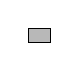
\begin{tikzpicture}[baseline=-2pt]\fill[black!28] (0,0) rectangle (0.28,0.18);\draw (0,0) rectangle (0.28,0.18);\end{tikzpicture}\quad
$E_{0,K}$: critical region, where $|\cos(2\pi q_0)|$ is small.

\medskip
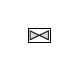
\begin{tikzpicture}[baseline=-2pt]
  \fill[white] (0,0) rectangle (0.28,0.18);
  \fill[black!15] (0.025,0.035) -- (0.14,0.09) -- (0.025,0.145) -- cycle;
  \fill[black!15] (0.255,0.035) -- (0.14,0.09) -- (0.255,0.145) -- cycle;
  \draw[black!85,line width=0.4pt] (0.025,0.035) -- (0.14,0.09) -- (0.025,0.145) -- cycle;
  \draw[black!85,line width=0.4pt] (0.255,0.035) -- (0.14,0.09) -- (0.255,0.145) -- cycle;
  \draw (0,0) rectangle (0.28,0.18);
\end{tikzpicture}\quad
$\T^2\setminus E_{0,K}$: good region, where the invariant cones are shown as hourglasses (opposite tangent-space sectors).

\medskip
\footnotesize The width of the strips decreases as the threshold $\eta_K$ decreases. The figure is schematic: it shows the geometry of the critical bands, not their exact width for a specific choice of threshold.
\end{minipage}
\caption{The one-step critical region $E_{0,K}$ and its complement. The bad region consists of two vertical strips around the critical lines $q_0=\tfrac14$ and $q_0=\tfrac34$, where $\cos(2\pi q_0)=0$. Outside these strips the derivative has a standard invariant cone field.}
\label{fig:E0K}
\end{figure}

\subsection*{The contradiction we aim to reach}
Suppose, toward a contradiction, that there is a sequence of parameters
$K_j\to\infty$ for which the top Lyapunov exponent of the standard map is
zero almost everywhere. For each parameter $K_j$, subadditivity and bounded
convergence imply that the normalized mean growth tends to zero as the time
length tends to infinity. Equivalently,
\begin{equation}\label{eq:long}
  \lim_{n\to\infty}e_n(K_j)=1\qquad\text{for every fixed }j.
\end{equation}
In the other direction, the proposition proved in the next section gives
\begin{equation}\label{eq:short}
  \lim_{j\to\infty}e_n(K_j)=0\qquad\text{for every fixed }n\ge1.
\end{equation}

\begin{center}
\setlength{\fboxsep}{9pt}%
\fbox{\begin{minipage}{0.89\textwidth}
\textbf{Target of the contradiction argument.}
Assume there exists a sequence $K_j\to\infty$ with zero Lyapunov exponent
a.e.\ at every $K_j$. Then one would have simultaneously
\[
 \boxed{\quad
 \underbrace{\lim_{n\to\infty}e_n(K_j)=1}_{\text{each fixed }j}
 \qquad\text{and}\qquad
 \underbrace{\lim_{j\to\infty}e_n(K_j)=0}_{\text{each fixed }n}.
 \quad}
\]
\textbf{Goal:} prove that no such sequence of parameters exists, by
combining the dynamical estimates (Theorems 3.1 and 5.1) with the geometric
multiscale argument of Sections 6--8.
\end{minipage}}
\end{center}

\textbf{Important logical point.} The two iterated limits alone are
compatible for a general function of $(n,K)$; the contradiction is supplied
by the additional structure of the standard-map cocycle.

\section{Proof that $e_n(K)\to0$ for fixed $n$}\label{sec:fixed}

\begin{fixedgrowth}
For every fixed integer $n\ge1$,
\begin{equation}\label{eq:claim}
 \boxed{\lim_{K\to\infty}e_n(K)=0.}
\end{equation}
Equivalently,
\[
 \lim_{K\to\infty}\EE\left[\frac{\log\norm{T_{0,n}(z)}}{n\log M}\right]=1.
\]
\end{fixedgrowth}

\begin{proof}
Fix $n\ge1$ and $\varepsilon\in(0,1)$. The argument consists of three steps.

\smallskip
\noindent\emph{Step 1: the finitely many coefficients are typically large.}
Define the event
\begin{equation}\label{eq:event}
 E_{n,K}=\bigl\{z:\ |v(q_i(z))|\ge M^{1-\varepsilon}\text{ for every }0\le i<n\bigr\}.
\end{equation}

We call $E_{n,K}$ the \emph{hyperbolic region} (good single-step growth),
and its complement $E_{n,K}^{\,c}$ the \emph{elliptic region} (at least one
small coefficient), as visual shorthand in the following diagram. These are
\emph{not} assertions about uniform hyperbolicity or actual elliptic periodic
orbits: the complement consists precisely of points where at least one of the
$n$ coefficients misses the stated threshold.

\begin{figure}[htbp]
\centering
\begin{minipage}[c]{0.50\textwidth}
\centering
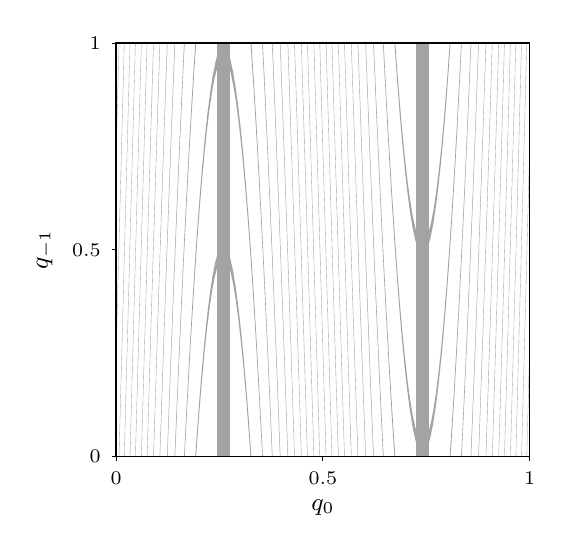
\begin{tikzpicture}[x=5.25cm,y=5.25cm]
  % True (not merely schematic) bad-coefficient strips for n=2.
  % K=36, epsilon=2/3; M=40, A=40^(1/3).
  % Bad q in (a,b) or (1-b,1-a) where
  % a=acos((A-2)/K)/(2*pi), b=acos((-A-2)/K)/(2*pi).
  \def\badA{0.24372}
  \def\badB{0.27406}
  \def\badC{0.72594}
  \def\badD{0.75628}
  \begin{scope}
    \clip (0,0) rectangle (1,1);
    \fill[white] (0,0) rectangle (1,1);
    % The preimages under (q_0,q_{-1}) -> q_1 of the two bad intervals.
    \foreach \m in {-8,...,8} {
      \foreach \qa/\qb in {0.24372/0.27406,0.72594/0.75628} {
        \path[fill=black!36]
          plot[domain=0:1,samples=160,variable=\xx]
            (\xx,{2*\xx+5.72957795*sin(360*\xx)-\qb-\m})
          -- plot[domain=1:0,samples=160,variable=\xx]
            (\xx,{2*\xx+5.72957795*sin(360*\xx)-\qa-\m})
          -- cycle;
      }
    }
    % Bad q_0-coefficient sets: exactly two vertical strips.
    \fill[black!36] (\badA,0) rectangle (\badB,1);
    \fill[black!36] (\badC,0) rectangle (\badD,1);
  \end{scope}
  \draw[line width=0.6pt] (0,0) rectangle (1,1);
  \foreach \x in {0,0.5,1}{
    \draw (\x,0) -- ++(0,-0.010);
    \node[below,font=\scriptsize] at (\x,-0.014) {$\x$};
  }
  \foreach \y in {0,0.5,1}{
    \draw (0,\y) -- ++(-0.010,0);
    \node[left,font=\scriptsize] at (-0.014,\y) {$\y$};
  }
  \node[below,font=\small] at (0.5,-0.082) {$q_0$};
  \node[above,rotate=90,font=\small] at (-0.13,0.5) {$q_{-1}$};
\end{tikzpicture}
\end{minipage}%
\hfill
\begin{minipage}[c]{0.45\textwidth}
\raggedright
\textbf{The torus as a unit square.}
Opposite sides are identified; each point is $(q_0,q_{-1})$.

\medskip
\begin{tikzpicture}[baseline=-2pt]\fill[white] (0,0) rectangle (0.28,0.18);\draw (0,0) rectangle (0.28,0.18);\end{tikzpicture}\quad
\textbf{Hyperbolic region} $E_{2,K}$:
all required coefficients are large.

\medskip
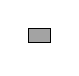
\begin{tikzpicture}[baseline=-2pt]\fill[black!36] (0,0) rectangle (0.28,0.18);\draw (0,0) rectangle (0.28,0.18);\end{tikzpicture}\quad
\textbf{Elliptic region} $E_{2,K}^{\,c}$:
one or more coefficients are small.

\medskip
\footnotesize Illustrative exact two-step geometry for $K=36$ and
$\varepsilon=2/3$. The curved bands are pullbacks of bad-coefficient strips.
\end{minipage}
\caption{Hyperbolic and elliptic regions (terminology used only for this
finite-time good/bad partition). For general $n$, the gray region is the union
of the pullbacks of the bad single-step strips at times $0,\ldots,n-1$.}
\label{fig:regions}
\end{figure}
For each fixed $i$, the position $q_i$ is uniformly distributed on $\T$, so
\begin{align}
\PP\bigl(|v(q_i)|<M^{1-\varepsilon}\bigr)
&\le\operatorname{Leb}\left\{q\in\T:\ |\cos(2\pi q)|
\le\frac{M^{1-\varepsilon}+2}{K}\right\}.
\end{align}
Since $M=K+4$,
\[
 \frac{M^{1-\varepsilon}+2}{K}\longrightarrow0,
\]
and the zero set of $\cos(2\pi q)$ has Lebesgue measure zero. Hence each probability on the left tends to zero. The union bound gives
\begin{equation}\label{eq:union}
 \PP(E_{n,K}^{\,c})\le\sum_{i=0}^{n-1}
 \PP\bigl(|v(q_i)|<M^{1-\varepsilon}\bigr)\longrightarrow0.
\end{equation}
This uses that $n$ is fixed; independence of the $q_i$ is unnecessary.

\smallskip
\noindent\emph{Step 2: large coefficients force almost maximal growth.}
Set $A=M^{1-\varepsilon}$. Consider the solution of \eqref{eq:linearization} with
\[
 u_0=1,\qquad u_{-1}=0.
\]
On $E_{n,K}$, all the coefficients $|v(q_j)|$ are at least $A$. Take $K$ large enough that $A-1\ge1$. We prove by induction that
\begin{equation}\label{eq:induction}
 |u_{j+1}|\ge(A-1)|u_j|\ge|u_j|,\qquad 0\le j<n.
\end{equation}
At $j=0$ it follows from $u_{-1}=0$. If $|u_{j-1}|\le|u_j|$, the recurrence gives
\begin{align*}
 |u_{j+1}|
 &=|v(q_j)u_j-u_{j-1}|\\
 &\ge |v(q_j)|\,|u_j|-|u_{j-1}|\\
 &\ge(A-1)|u_j|.
\end{align*}
As $A-1\ge1$, the induction continues. Therefore $|u_n|\ge(A-1)^n$. Since $T_{0,n}$ sends the unit vector $(1,0)$ to $(u_n,u_{n-1})$,
\begin{equation}\label{eq:large-transfer}
 \norm{T_{0,n}}\ge |u_n|\ge(M^{1-\varepsilon}-1)^n
 \qquad\text{on }E_{n,K}.
\end{equation}
Consequently,
\begin{equation}\label{eq:finite-lower}
 \frac{g(0,n)}n\ge\log_M(M^{1-\varepsilon}-1)
 \longrightarrow1-\varepsilon
 \qquad(K\to\infty)
\end{equation}
on this event.

\smallskip
\noindent\emph{Step 3: average the shortfall.}
Since $0\le1-g(0,n)/n\le1$ everywhere, split the expectation between $E_{n,K}$ and its complement. Equations \eqref{eq:union} and \eqref{eq:finite-lower} yield
\begin{align*}
 e_n(K)
 &=\EE\left[1-\frac{g(0,n)}n\right]\\
 &\le1-\log_M(M^{1-\varepsilon}-1)+\PP(E_{n,K}^{\,c}).
\end{align*}
Taking the upper limit as $K\to\infty$,
\[
 0\le\limsup_{K\to\infty}e_n(K)\le\varepsilon.
\]
Because $\varepsilon>0$ is arbitrary, the conclusion \eqref{eq:claim} follows.
\end{proof}

\paragraph{What this proof uses.}
Only the explicit coefficient $v(q)=2+K\cos(2\pi q)$, uniform one-time marginals, the union bound for finitely many times, and a deterministic induction for the recurrence. Neither Theorem 3.1 nor Theorem 5.1 is needed for this fixed-time statement.

\section{Theorem 3.1: cancellation is exponentially rare}

\begin{cancellation}
There exist constants $\delta>0$, $C<\infty$, $\gamma>0$, and $M_0<\infty$ such that, for all $M\ge M_0$, $i\in\Z$, and $n\ge1$,
\begin{equation}\label{eq:cancel}
\boxed{\begin{aligned}
\PP\bigl\{\;&\min\{g(i-n,i),g(i,i+n)\}\ge(1-\delta)n,\\[-2pt]
           &g(i-n,i+n)\le\delta n\bigr\}
\le Ce^{-\gamma n}.
\end{aligned}}
\end{equation}
All four constants are independent of $M$, $i$, and $n$ in the indicated range.
\end{cancellation}

\paragraph{Meaning.} Both half-intervals have nearly maximal growth, but their concatenation almost completely cancels. Such cancellation is algebraically possible in $\mathrm{SL}(2,\R)$, yet for the standard map the set of initial conditions producing it has exponentially small area.

\paragraph{Proof mechanism (Sections 3--4).} When the event in \eqref{eq:cancel} occurs, the expanding directions for the forward and backward products must be extremely close. Taking an appropriate perpendicular direction produces a nontrivial solution of the linearized recurrence that is exponentially small at both distant endpoints. The large-growth assumption then provides many matched, well-expanding scales after excluding the comparatively few poor-growth locations. At each such scale an analytic \emph{local scarcity} estimate restricts the allowed values of a transverse initial coordinate. Iteration over linearly many matched scales gives the factor $e^{-\gamma n}$. The local analytic estimate is the substantive work of Section 4.

\section{Theorem 5.1: a product estimate across a fast bridge}

\subsection*{Observations}
For distinct integer times $d,e$, introduce the \emph{normalized shortfall}
\begin{equation}\label{eq:obssh}
 \mathfrak h_{d,e}(z)=1-\frac{g(d,e;z)}{|d-e|}\in[0,1].
\end{equation}
This is a finite-time random variable on the phase-space torus. A function
of a controlled number of such variables is an \emph{observation}.

\begin{observationdef}
Fix an integer $R\ge1$ and constants $L,B\ge0$. An
\textbf{observation with bounds $(R,L,B)$} is a real-valued function
$O:\T^2\to\R$ that can be expressed as
\begin{equation}\label{eq:observation-def}
 O(z)=F\bigl(\mathfrak h_{d_1,e_1}(z),\ldots,
             \mathfrak h_{d_r,e_r}(z)\bigr),\qquad 0\le r\le R,
\end{equation}
where $d_\ell,e_\ell\in\Z$, $d_\ell\ne e_\ell$, and where the defining
function $F:[0,1]^r\to\R$ satisfies
\begin{equation}\label{eq:observation-bounds}
 \sup_{u\in[0,1]^r}|F(u)|\le B,
 \qquad
 |F(u)-F(v)|\le L\,\norm{u-v}_\infty
 \quad (u,v\in[0,1]^r).
\end{equation}
The case $r=0$ is understood as a constant observation.
The set of \emph{indices used by the observation} is
$\{d_1,e_1,\ldots,d_r,e_r\}$.
\end{observationdef}

\textbf{Points to note.}
The integer pairs, the number of arguments $r$, and even $F$ may change
with the parameter or with an application; the common bounds $(R,L,B)$
remain fixed. The definition places no sign condition on $O$. For example,
$O(z)=\mathfrak h_{p,q}(z)$ is a $(1,1,1)$-observation; so is
$O(z)=1-\mathfrak h_{p,q}(z)$. By contrast, an indicator such as
$\one_{\{\mathfrak h_{p,q}>h\}}$ is generally not a Lipschitz observation.
The theorem instead uses the indicator $\one_{\{H>h\}}$ \emph{of an event
specified by} an observation $H$.

An observation is \emph{localized near} time $a$ on scale $n$ if
$|d_\ell-a|,|e_\ell-a|\le\kappa n$ for all its indices. Theorem 5.1
concerns two such localized observations at the two ends of a long interval.
The Lipschitz condition ensures that changing each underlying shortfall by
at most $\eta$ changes the value of the observation by at most $L\eta$;
this is needed to transport observations along contracting graphs.

\begin{bridge}
There are absolute constants $c_b\in(0,1)$, $\kappa>0$, and $\sigma>0$ with the following property. Fix bounds $(R,L,B)$ and $h>0$. For sufficiently large $M$ and $n=b-a$, let $W,H$ be observations with these bounds, with $W\ge0$. Suppose all indices defining one observation lie within $\kappa n$ of $a$, and those defining the other lie within $\kappa n$ of $b$; either assignment is allowed. Then
\begin{equation}\label{eq:bridge}
\boxed{\begin{aligned}
&\EE\left[\one_{\{g(a,b)\ge c_b n\}}\,W\,\one_{\{H>h\}}\right]\\
&\hspace{13mm}\le C\left(\EE W+M^{-\sigma n}\right)\PP(H>h/2).
\end{aligned}}
\end{equation}
Here $C$ and the thresholds for sufficiently large $M,n$ may depend on $(R,L,B)$ and $h$, but not on the bridge location, indices, or specific defining functions.
\end{bridge}

\paragraph{Meaning.} The condition $g(a,b)\ge c_b(b-a)$ says that the connecting interval is a \emph{fast bridge}. On such an interval, the theorem gives a weighted decorrelation inequality for observations placed near opposite endpoints. Schematically, ignoring the threshold relaxation and the small error,
\[
 \EE\bigl[\one_{\{\text{fast bridge}\}}W\one_{\{H>h\}}\bigr]
 \ \lesssim\ \EE W\,\PP(H>h).
\]
This is \emph{not} an assumption that the two observations are independent, and it is not an unconditional mixing statement.

\paragraph{Proof mechanism (Section 5).} Strong growth along the bridge gives many middle times with good forward and backward expansion. Finite Dirichlet boundary-value problems construct two transverse families of contracting graphs. Along an appropriate contracting graph, one endpoint observation varies very little. Uniform distortion estimates for the graph Jacobians, followed by changes of variables and integration along the two transverse families, yield the product inequality.

\medskip
\noindent\textbf{Difference between the two estimates.}
Theorem 3.1 rules out excessive cancellation of two large products; Theorem 5.1 controls the joint occurrence of endpoint observations across a strongly expanding interval. They are separate dynamical inputs to the later multiscale argument.

\section{How the ingredients fit together}

The central tension is between \eqref{eq:short}, which describes almost-maximal growth at every fixed time as $K$ increases, and \eqref{eq:long}, which describes vanishing average exponential growth at long times under the zero-exponent hypothesis. Section 6 chooses an intermediate dyadic range at which the shortfall first becomes appreciable. The cancellation estimate controls jumps in the shortfall across scales, while the bridge estimate constrains the geometry of possible limit distance arrays. Sections 7--8 then use those constraints in the geometric balance argument to reach a contradiction.

\begin{center}
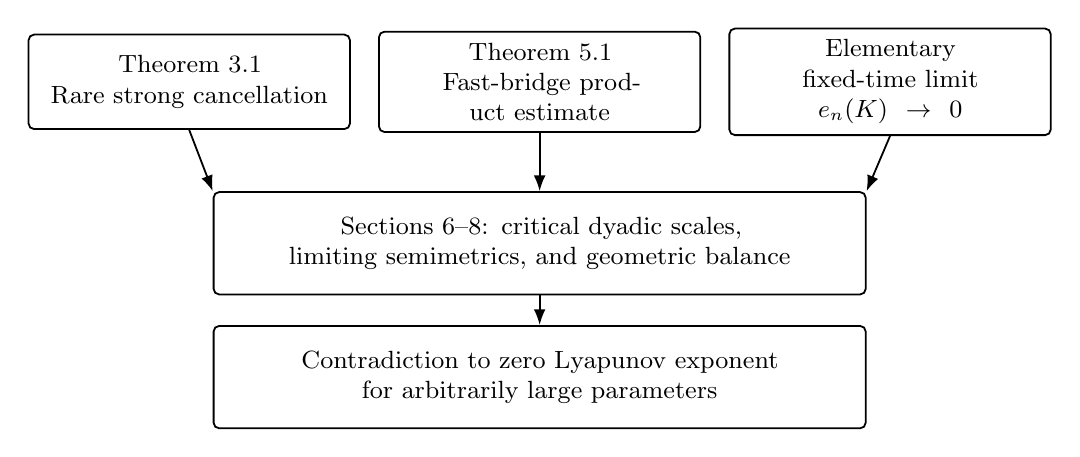
\begin{tikzpicture}[
  every node/.style={font=\small,align=center},
  ingredient/.style={draw,rounded corners=2pt,minimum height=12mm,text width=38mm,inner sep=4pt},
  downstream/.style={draw,rounded corners=2pt,minimum height=13mm,text width=80mm,inner sep=4pt},
  >={Latex[length=2mm]},
  every path/.style={line width=0.65pt}
]
  \node[ingredient] (can) at (-4.45,0) {Theorem 3.1\\Rare strong cancellation};
  \node[ingredient] (bridge) at (0,0) {Theorem 5.1\\Fast-bridge product estimate};
  \node[ingredient] (fixed) at (4.45,0) {Elementary fixed-time limit\\$e_n(K)\to0$};
  \node[downstream] (geom) at (0,-2.05) {Sections 6--8: critical dyadic scales,\\limiting semimetrics, and geometric balance};
  \node[downstream] (contr) at (0,-3.75) {Contradiction to zero Lyapunov exponent\\for arbitrarily large parameters};
  \draw[->] (can.south) -- (geom.north west);
  \draw[->] (bridge.south) -- (geom.north);
  \draw[->] (fixed.south) -- (geom.north east);
  \draw[->] (geom.south) -- (contr.north);
\end{tikzpicture}
\end{center}

\paragraph{Reference.} OpenAI, \emph{Positive Metric Entropy for the Standard Map at Large Parameters}, preprint, 23 September 2026, especially Sections 1--6.\newline
\url{https://github.com/openai/math/tree/main/preprints/Positive-Metric-Entropy-for-the-Standard-Map-at-Large-Parameters-September-23-2026}

\end{document}
